\documentclass[12pt,a4paper,oneside]{abntspiifac}

% ---- Codificação e língua ----
\usepackage[utf8]{inputenc}
\usepackage[T1]{fontenc}
\usepackage[brazil]{babel}

% ---- Fontes ----
\usepackage{mathptmx}

% ---- Pacotes gráficos e tabelas ----
\usepackage{graphicx}
\usepackage{float}
\usepackage{booktabs}
\usepackage{longtable}
\usepackage{array}
\usepackage{multirow}
\usepackage{tabularx}
\usepackage{xcolor}

% ---- Pacotes de layout ----
\usepackage{indentfirst}
\usepackage{microtype}
\usepackage{lastpage}

% ---- Citações ABNT ----
\usepackage[alf,abnt-emphasize=bf,abnt-etal-list=3,abnt-etal-text=it]{abntex2cite}

% ---- Configurações de PDF ----
\hypersetup{
  pdftitle={Projeto de TCC: SIGEI},
  pdfauthor={Euzébio do Nascimento Oliveira Neto},
  pdfsubject={Projeto de Trabalho de Conclusão de Curso},
  pdfkeywords={SIGEI, Escolas Indígenas, Sistema de Informação, Georreferenciamento},
  colorlinks=false
}

% METADADOS

\instituicao{Instituto Federal de Educação, Ciência e Tecnologia do Acre}
\campus{Campus Rio Branco}
\programa{Curso Superior de Tecnologia em Análise e Desenvolvimento de Sistemas}

\autor{Euzébio do Nascimento Oliveira Neto}
\autorVirg{Oliveira Neto, Euzébio do Nascimento}

\titulo{SIGEI}
\subtitulo{Sistema de Gerenciamento Escolar Indígena}

\natureza{Projeto de Trabalho de Conclusão de Curso apresentado ao Curso Superior de Tecnologia em Análise e Desenvolvimento de Sistemas do Instituto Federal de Educação, Ciência e Tecnologia do Acre, como requisito parcial para aprovação na disciplina de Metodologia Científica e Tecnológica.}

\orientadorTitulo{Prof. Me.}
\orientador{Marlon Amaro Coelho Teixeira}

\objeto{Projeto de Trabalho de Conclusão de Curso}
\finalcatalog{1. Sistemas de informação. 2. Educação indígena. 3. Georreferenciamento. 4. Desenvolvimento web. I. Título.}

\local{Rio Branco}
\data{2026}

\begin{document}

\pretextual

% -- Capa --
\inserecapa

% -- Folha de rosto --
\inserefolhaderosto{Folha de rosto}

% ---- Lista de abreviaturas e siglas ----
\begin{siglas}
  \item[ABNT]   Associação Brasileira de Normas Técnicas
  \item[AEE]    Atendimento Educacional Especializado
  \item[API]    \textit{Application Programming Interface}
  \item[CORS]   \textit{Cross-Origin Resource Sharing}
  \item[CRUD]   \textit{Create, Read, Update, Delete}
  \item[CSS]    \textit{Cascading Style Sheets}
  \item[DTO]    \textit{Data Transfer Object}
  \item[EJA]    Educação de Jovens e Adultos
  \item[FUNAI]  Fundação Nacional dos Povos Indígenas
  \item[HTML]   \textit{HyperText Markup Language}
  \item[HTTP]   \textit{HyperText Transfer Protocol}
  \item[IBGE]   Instituto Brasileiro de Geografia e Estatística
  \item[IFAC]   Instituto Federal de Educação, Ciência e Tecnologia do Acre
  \item[INEP]   Instituto Nacional de Estudos e Pesquisas Educacionais Anísio Teixeira
  \item[JPA]    \textit{Java Persistence API}
  \item[JSON]   \textit{JavaScript Object Notation}
  \item[JWT]    \textit{JSON Web Token}
  \item[LDB]    Lei de Diretrizes e Bases da Educação Nacional
  \item[MEC]    Ministério da Educação
  \item[OIT]    Organização Internacional do Trabalho
  \item[ORM]    \textit{Object-Relational Mapping}
  \item[REST]   \textit{Representational State Transfer}
  \item[RF]     Requisito Funcional
  \item[RNF]    Requisito Não Funcional
  \item[SEE/AC] Secretaria de Estado de Educação, Cultura e Esportes do Acre
  \item[SIG]    Sistema de Informação Geográfica
  \item[SIGEI]  Sistema de Gerenciamento Escolar Indígena
  \item[SPA]    \textit{Single Page Application}
  \item[SQL]    \textit{Structured Query Language}
  \item[TCC]    Trabalho de Conclusão de Curso
  \item[UML]    \textit{Unified Modeling Language}
  \item[URL]    \textit{Uniform Resource Locator}
\end{siglas}

% ---- Sumário ----
\tableofcontents*
\cleardoublepage

\textual

% CAPÍTULO 1 — INTRODUÇÃO

\chapter{INTRODUÇÃO}
\label{cap:introducao}

O Estado do Acre, situado na região Norte do Brasil, abriga uma das populações indígenas mais expressivas do país em termos de diversidade cultural e linguística. A Fundação Nacional dos Povos Indígenas registra no estado a presença de mais de uma dezena de etnias distintas, distribuídas por territórios demarcados que, em sua maioria, localizam-se em áreas remotas, de acesso difícil e com infraestrutura de comunicação limitada \cite{brasil1988}. Essa realidade geográfica e sociocultural impõe desafios históricos ao poder público, especialmente no que diz respeito à oferta e ao gerenciamento da educação escolar destinada a esses povos.

A educação escolar indígena, garantida pela Constituição Federal de 1988 e regulamentada pela Lei de Diretrizes e Bases da Educação Nacional (Lei n.º 9.394/1996), prevê o ensino ministrado nas línguas maternas das comunidades, o respeito às especificidades culturais de cada povo e a participação ativa das próprias comunidades na gestão de suas escolas \cite{brasil1996}. No Acre, essa modalidade educacional é administrada pela Secretaria de Estado de Educação, Cultura e Esportes (SEE/AC), responsável pela coordenação de escolas distribuídas por municípios cujo acesso frequentemente depende de transporte fluvial ou de estradas em precário estado de conservação.

Diante da amplitude territorial e da diversidade das comunidades atendidas, a SEE/AC deparava-se, até o início do desenvolvimento deste projeto, com uma gestão fragmentada das informações escolares. Os dados referentes às 149 escolas indígenas e 19 anexos escolares existentes no estado encontravam-se dispersos em planilhas eletrônicas, documentos físicos e registros administrativos desconexos, sem integração entre si. Essa realidade dificultava a realização de consultas rápidas, a atualização cadastral, o cruzamento de informações e a emissão de relatórios gerenciais precisos, comprometendo a eficiência administrativa e a capacidade de planejamento educacional.

\section{Problema de Pesquisa}

A ausência de uma ferramenta tecnológica integrada para o gerenciamento das escolas indígenas do Acre gera inconsistências nos dados, retrabalho por parte dos gestores e dificuldades na tomada de decisões estratégicas. Como é possível, portanto, centralizar, organizar e disponibilizar de forma georreferenciada as informações das escolas indígenas acreanas, de modo a subsidiar a gestão educacional realizada pela SEE/AC?

\section{Justificativa}
\label{sec:justificativa}

A gestão eficiente de sistemas educacionais depende, em larga medida, da qualidade e da acessibilidade das informações disponíveis para seus gestores. Conforme destacam \citeonline{laudon2014}, os sistemas de informação desempenham papel central nas organizações contemporâneas ao fornecer dados estruturados que apoiam processos decisórios em todos os níveis hierárquicos. No contexto das escolas indígenas, essa necessidade é ainda mais premente, dado o isolamento geográfico das instituições e a complexidade administrativa inerente à gestão de múltiplas etnias, línguas e territórios.

A inexistência de uma plataforma digital integrada para o gerenciamento das escolas indígenas do Acre representa não apenas um obstáculo operacional, mas também um entrave ao exercício pleno do direito à educação diferenciada, assegurado constitucional e legalmente aos povos indígenas \cite{brasil1988}. Nesse sentido, o desenvolvimento do SIGEI justifica-se tanto pela necessidade técnica de modernização dos processos administrativos da SEE/AC quanto pelo potencial impacto social que a melhoria da gestão educacional pode trazer às comunidades beneficiadas.

A incorporação de funcionalidades de georreferenciamento ao sistema representa um diferencial estratégico, uma vez que permite a visualização espacial das escolas no território acreano, facilitando o planejamento logístico, a alocação de recursos humanos e materiais, e o monitoramento das condições de atendimento em cada unidade escolar \cite{longley2013}. Conforme \citeonline{camara2001}, a integração de dados geográficos com informações descritivas em sistemas de informação geográfica possibilita análises que seriam inviáveis em representações puramente tabulares, tornando o georreferenciamento uma ferramenta estratégica para a gestão de redes escolares dispersas geograficamente.

Do ponto de vista acadêmico, o projeto contribui para a área de Análise e Desenvolvimento de Sistemas ao demonstrar a aplicação prática de tecnologias modernas de desenvolvimento web — Angular, Spring Boot e PostgreSQL — na solução de problemas concretos da administração pública educacional, integrando aspectos de engenharia de software, sistemas de informação e ciência da geoinformação.

\section{Objetivo Geral}
\label{sec:objetivogeral}

Desenvolver uma plataforma web capaz de centralizar e gerenciar informações das escolas indígenas do Acre, proporcionando maior organização, rastreabilidade, eficiência administrativa e suporte à tomada de decisões por parte dos gestores da SEE/AC.

\section{Objetivos Específicos}
\label{sec:objetivosespecificos}

Para atingir o objetivo geral proposto, foram estabelecidos os seguintes objetivos específicos:

\begin{alineas}
  \item mapear geograficamente as escolas indígenas do Acre por meio de um mapa interativo;
  \item centralizar dados escolares, incluindo informações administrativas, pedagógicas e estruturais;
  \item facilitar consultas e atualizações cadastrais referentes a escolas, aldeias, municípios e terras indígenas;
  \item disponibilizar informações consolidadas para gestores educacionais por meio de relatórios gerenciais;
  \item reduzir inconsistências e retrabalho no gerenciamento de dados educacionais.
\end{alineas}

\section{Estrutura do Projeto}

O presente projeto encontra-se organizado em cinco seções principais. O Capítulo 1 apresenta a introdução, contextualizando o problema, a justificativa e os objetivos do estudo. O Capítulo 2 desenvolve a revisão de literatura, fornecendo a fundamentação teórica que embasa o sistema. O Capítulo 3 descreve os materiais e métodos adotados no desenvolvimento. O Capítulo 4 apresenta o desenvolvimento do sistema e os resultados obtidos. O Capítulo 5 apresenta o cronograma de execução. Por fim, são listadas as referências bibliográficas utilizadas.


% CAPÍTULO 2 — REVISÃO DE LITERATURA

\chapter{REVISÃO DE LITERATURA}
\label{cap:revisao}

Este capítulo apresenta os fundamentos teóricos que sustentam o desenvolvimento do SIGEI, abrangendo as áreas de sistemas de informação, gestão escolar, educação escolar indígena, sistemas de informação geográfica, georreferenciamento e as principais tecnologias de desenvolvimento web a serem utilizadas no projeto.

\section{Sistemas de Informação}

\subsection{Conceitos Fundamentais}

Um sistema de informação pode ser definido como um conjunto de componentes inter-relacionados que coletam, processam, armazenam e distribuem informações para apoiar a tomada de decisões, a coordenação, o controle, a análise e a visualização em uma organização \cite{laudon2014}. Segundo \citeonline{stair2015}, os sistemas de informação são constituídos por dados brutos que, após processados, transformam-se em informações com valor agregado para os usuários. Essa transformação ocorre por meio de processos de entrada, processamento e saída, que podem ser retroalimentados por mecanismos de controle e avaliação.

\citeonline{obrien2013} categorizam os sistemas de informação segundo seu nível organizacional de aplicação, distinguindo sistemas de processamento de transações, sistemas de suporte à decisão, sistemas de informações gerenciais e sistemas de suporte executivo. No contexto do SIGEI, o sistema enquadra-se predominantemente na categoria de sistema de informações gerenciais, uma vez que tem por finalidade consolidar dados operacionais das escolas indígenas e disponibilizá-los em formato adequado à tomada de decisões pelos gestores da SEE/AC.

\subsection{Importância para Organizações Públicas}

No setor público, os sistemas de informação assumem papel particularmente relevante ao possibilitar a modernização dos processos administrativos, a transparência na gestão e a melhoria nos serviços prestados à sociedade. \citeonline{laudon2014} ressaltam que as organizações que investem em sistemas de informação robustos tendem a apresentar maior eficiência operacional, melhor qualidade no processo decisório e maior capacidade de adaptação às mudanças no ambiente externo.

No contexto educacional, os sistemas de informação permitem a gestão integrada de dados relativos a matrículas, infraestrutura escolar e dados institucionais, contribuindo para o planejamento estratégico e a avaliação de políticas públicas. A disponibilidade de informações precisas e atualizadas é condição indispensável para que gestores educacionais possam identificar demandas, alocar recursos de forma eficiente e monitorar o alcance dos objetivos institucionais \cite{obrien2013}.

\section{Gestão Escolar}

\subsection{Conceitos e Abrangência}

A gestão escolar compreende o conjunto de atividades administrativas e pedagógicas que visam assegurar o funcionamento adequado das instituições de ensino, garantindo condições favoráveis ao processo de ensino e aprendizagem \cite{libaneofernandes2012}. Segundo \citeonline{luck2009}, a gestão escolar eficaz pressupõe a articulação entre dimensões pedagógicas, administrativas, financeiras e de relacionamento comunitário, demandando dos gestores competências diversas e o domínio de ferramentas adequadas para a organização institucional.

No âmbito administrativo, a gestão escolar envolve o controle de matrículas, o acompanhamento da infraestrutura física das escolas e a prestação de contas aos órgãos reguladores. Tais atividades, quando realizadas sem o suporte de sistemas informacionais adequados, tendem a gerar sobrecarga de trabalho, inconsistências nos registros e dificuldades no cumprimento das obrigações legais \cite{libaneofernandes2012}.

\subsection{Desafios Administrativos na Gestão Escolar Indígena}

A gestão de escolas indígenas apresenta desafios específicos que a distinguem da administração de escolas convencionais. A dispersão geográfica das comunidades, a diversidade linguística e cultural, a irregularidade no acesso às tecnologias de comunicação e as particularidades dos calendários escolares adaptados ao ritmo das comunidades são fatores que complexificam o gerenciamento dessas instituições \cite{grupioni2006}.

Além disso, a gestão escolar indígena frequentemente envolve a articulação entre o poder público estadual, as lideranças comunitárias indígenas, o Ministério da Educação e a Fundação Nacional dos Povos Indígenas, exigindo fluxos de comunicação e registros documentais que demandam organização sistemática e eficiente \cite{brasil2012}.

\section{Educação Escolar Indígena}

\subsection{Aspectos Legais}

A educação escolar indígena no Brasil é assegurada por um conjunto de dispositivos legais que historicamente representaram avanço significativo no reconhecimento dos direitos dos povos originários. A Constituição Federal de 1988, em seus artigos 210, 215 e 231, reconhece aos povos indígenas a organização social, os costumes, as línguas, as crenças e as tradições, bem como o direito à educação ministrada em suas línguas maternas e com processos próprios de aprendizagem \cite{brasil1988}.

A Lei de Diretrizes e Bases da Educação Nacional (Lei n.º 9.394/1996), em seu artigo 78, estabelece a obrigação do Estado de oferecer educação escolar bilíngue e intercultural aos povos indígenas, com currículos e programas específicos que incluam seus conteúdos culturais \cite{brasil1996}. A Resolução CNE/CEB n.º 5/2012 define as Diretrizes Curriculares Nacionais para a Educação Escolar Indígena na Educação Básica, consolidando os princípios de interculturalidade, bilinguismo e especificidade que devem orientar a oferta educacional para as comunidades indígenas \cite{brasil2012}.

No plano internacional, a Convenção n.º 169 da Organização Internacional do Trabalho (OIT), promulgada no Brasil pelo Decreto n.º 5.051/2004, reafirma o direito dos povos indígenas e tribais à educação em todos os seus níveis, respeitando suas especificidades culturais e linguísticas \cite{brazil2004}.

\subsection{Particularidades da Gestão da Educação Indígena no Acre}

O Acre abriga um mosaico de povos indígenas que inclui, entre outros, os Ashaninka, Jaminawa, Kaxinawá (Huni Kuin), Manchineri, Nukini e Yawanapi. Esses povos habitam territórios demarcados distribuídos por municípios como Cruzeiro do Sul, Feijó, Jordão, Marechal Thaumaturgo, Santa Rosa do Purus e Tarauacá, além da capital Rio Branco \cite{secretariaacre2022}.

A gestão das escolas indígenas acreanas pela SEE/AC envolve a coordenação de unidades escolares localizadas em territórios de acesso restrito e a adaptação dos currículos às realidades culturais e linguísticas de cada povo. Conforme \citeonline{munduruku2019}, a educação indígena não pode ser tratada como mera extensão da educação não indígena, sendo necessário o desenvolvimento de ferramentas e metodologias adequadas às especificidades de cada contexto cultural.

\section{Sistemas de Informação Geográfica}

\subsection{Conceitos}

Um Sistema de Informação Geográfica (SIG) é definido como um conjunto integrado de hardware, software, dados e metodologias destinado à coleta, armazenamento, recuperação, análise e exibição de dados espacialmente referenciados \cite{longley2013}. Segundo \citeonline{camara2001}, os SIGs distinguem-se de outros sistemas de informação pela sua capacidade de integrar dados de natureza geográfica com informações descritivas, permitindo análises espaciais que revelam padrões e relações não perceptíveis em representações puramente tabulares.

Os componentes essenciais de um SIG incluem: dados espaciais (geometrias representando entidades do mundo real), dados de atributos (informações descritivas associadas às entidades geográficas), ferramentas de análise espacial e interfaces de visualização, como mapas digitais interativos \cite{longley2013}.

\subsection{Aplicações Educacionais}

No campo educacional, os SIGs têm sido utilizados crescentemente para subsidiar o planejamento e a avaliação de redes de ensino. Segundo \citeonline{moura2003}, a representação cartográfica de estabelecimentos educacionais permite identificar lacunas na cobertura territorial do atendimento escolar, otimizar rotas de transporte estudantil e diagnosticar desigualdades regionais no acesso à educação.

No contexto das escolas indígenas, a incorporação de funcionalidades geográficas a sistemas de gestão educacional possibilita a visualização da distribuição espacial das unidades escolares nos territórios demarcados, facilitando o planejamento de visitas técnicas e a identificação de comunidades sem cobertura educacional adequada \cite{camara2001}.

\section{Georreferenciamento}

O georreferenciamento consiste no processo de associação de dados ou objetos a uma localização geográfica específica, expressa por coordenadas geográficas — latitude e longitude — ou por um sistema de referência espacial definido \cite{moura2003}. Essa técnica permite que informações de natureza diversa, como escolas, aldeias e infraestruturas, sejam representadas em mapas digitais e submetidas a análises espaciais.

Para o SIGEI, o georreferenciamento das escolas indígenas representa uma funcionalidade central, pois permite que os gestores da SEE/AC visualizem a distribuição geográfica das unidades escolares no território acreano e relacionem essa informação espacial com dados administrativos, como o número de matrículas e a situação da infraestrutura. Conforme \citeonline{longley2013}, a combinação de dados geoespaciais com atributos descritivos constitui a base para análises de suporte à decisão em organizações que operam em territórios amplos e geograficamente diversificados.

\section{Tecnologias de Desenvolvimento Web}

\subsection{Angular}

Angular é um framework de desenvolvimento de aplicações web mantido pela Google, construído sobre a linguagem TypeScript. Trata-se de uma plataforma completa para o desenvolvimento de aplicações de página única (\textit{Single Page Applications} — SPA), oferecendo um conjunto integrado de ferramentas para gerenciamento de estado, roteamento, comunicação com servidores e construção de componentes reutilizáveis \cite{fain2017}.

A arquitetura do Angular baseia-se no padrão de componentes, em que cada elemento da interface do usuário é encapsulado em um componente com seu próprio template HTML, folha de estilos CSS e lógica TypeScript. A comunicação entre componentes é gerenciada por meio de serviços injetáveis responsáveis pelo compartilhamento de dados e pela comunicação com APIs externas \cite{freeman2019}.

\subsection{Spring Boot}

Spring Boot é um framework baseado no ecossistema Spring para a plataforma Java, projetado para simplificar o desenvolvimento de aplicações web e microsserviços. Sua principal característica é a configuração automática (\textit{auto-configuration}), que reduz significativamente a quantidade de código necessário para iniciar uma aplicação \cite{walls2019}. O Spring Boot integra-se nativamente com o Spring Data JPA para o acesso a dados relacionais por meio de repositórios baseados em interfaces, com o Hibernate como implementação padrão do JPA, permitindo o mapeamento objeto-relacional entre as entidades Java e as tabelas do banco de dados \cite{bauer2015}.

\subsection{PostgreSQL}

PostgreSQL é um sistema gerenciador de banco de dados relacional de código aberto, reconhecido por sua robustez, conformidade com os padrões SQL e suporte a tipos de dados avançados \cite{obe2017}. Conforme \citeonline{postgresql2023}, o sistema oferece recursos como transações ACID, controle de concorrência por versionamento de linhas (MVCC) e índices de múltiplos tipos, fazendo dele uma escolha sólida para aplicações que demandam integridade de dados e desempenho em cenários de alta concorrência.

\subsection{API REST}

REST (\textit{Representational State Transfer}) é um estilo arquitetural para o desenvolvimento de serviços web proposto por \citeonline{fielding2000}. As APIs RESTful utilizam o protocolo HTTP, adotando os verbos \texttt{GET}, \texttt{POST}, \texttt{PUT} e \texttt{DELETE} para expressar as operações sobre os recursos expostos. São caracterizadas pela ausência de estado nas requisições, pela utilização de identificadores uniformes de recursos (URIs) e pela representação dos recursos em formatos padronizados como JSON \cite{richardson2013}.

\subsection{Leaflet}

Leaflet é uma biblioteca JavaScript de código aberto voltada para o desenvolvimento de mapas interativos em aplicações web. Projetada com foco em leveza e desempenho, oferece suporte a camadas de mapeamento baseadas em \textit{tiles}, marcadores, \textit{pop-ups} e outros elementos cartográficos, sendo compatível com o OpenStreetMap \cite{leaflet2023}. No contexto do SIGEI, o Leaflet será utilizado para renderizar o mapa interativo que exibirá a localização georreferenciada das escolas indígenas do Acre, com marcadores posicionados segundo as coordenadas geográficas cadastradas no banco de dados \cite{muehlenhaus2014}.


% CAPÍTULO 3 — MATERIAL E MÉTODOS

\chapter{MATERIAL E MÉTODOS}
\label{cap:metodos}

Este capítulo descreve os procedimentos metodológicos a serem adotados no desenvolvimento do SIGEI, abrangendo o tipo de pesquisa, a metodologia de desenvolvimento, o levantamento de requisitos, a modelagem prevista e a arquitetura tecnológica planejada.

\section{Tipo de Pesquisa}

Do ponto de vista de sua natureza, o presente trabalho caracteriza-se como uma pesquisa aplicada, uma vez que objetiva gerar conhecimentos direcionados à solução de um problema prático específico: a ausência de um sistema integrado para o gerenciamento das escolas indígenas do Acre \cite{gil2008}. Segundo \citeonline{wazlawick2013}, pesquisas aplicadas na área de Ciência da Computação envolvem o desenvolvimento de artefatos tecnológicos — como sistemas de software, \textit{frameworks} ou algoritmos — que respondem a demandas identificadas em contextos reais de uso.

Quanto aos objetivos, o estudo apresenta caráter descritivo-exploratório, na medida em que descreverá as funcionalidades do sistema desenvolvido e explorará as potencialidades das tecnologias adotadas para a solução do problema de gestão identificado \cite{gil2008}.

\section{Metodologia de Desenvolvimento}

O SIGEI será desenvolvido por meio de uma metodologia incremental, na qual o sistema será construído de forma progressiva, com cada incremento representando um conjunto coeso de funcionalidades testadas e integradas ao produto final \cite{pressman2016}. Essa abordagem permitirá a entrega contínua de valor e possibilitará a identificação e a correção precoce de desvios em relação aos requisitos levantados.

O processo de desenvolvimento será organizado nas seguintes fases:

\begin{alineas}
  \item \textbf{Levantamento de requisitos:} identificação das necessidades dos usuários por meio de reuniões com profissionais da SEE/AC, análise de documentos existentes e observação dos processos de trabalho vigentes;
  \item \textbf{Modelagem:} elaboração dos diagramas de casos de uso, entidade-relacionamento e da arquitetura em camadas do sistema;
  \item \textbf{Implementação incremental:} desenvolvimento iterativo do \textit{backend}, do \textit{frontend} e do banco de dados, com integração contínua entre os módulos;
  \item \textbf{Testes:} verificação funcional de cada módulo implementado, com correção de falhas identificadas;
  \item \textbf{Implantação:} configuração do ambiente de execução e disponibilização do sistema para uso pelos gestores da SEE/AC.
\end{alineas}

\section{Levantamento de Requisitos}

O levantamento de requisitos constitui etapa fundamental no desenvolvimento de sistemas de informação, pois é nessa fase que as necessidades dos usuários são identificadas e traduzidas em especificações formais que orientam a construção do \textit{software} \cite{sommerville2019}. Para o SIGEI, os requisitos foram identificados por meio de reuniões com representantes da SEE/AC, análise de planilhas de dados existentes e estudo da legislação pertinente à educação escolar indígena.

Os requisitos foram classificados em funcionais, que descrevem as funções que o sistema deve realizar, e não funcionais, que expressam restrições e qualidades que o sistema deve apresentar \cite{pressman2016}.

\subsection{Requisitos Funcionais}

Os requisitos funcionais do SIGEI são apresentados no Quadro~\ref{qua:rf}.

\begin{longtable}{p{1.5cm}p{4.5cm}p{7.5cm}}
\caption{Requisitos Funcionais do SIGEI}
\label{qua:rf} \\
\toprule
\textbf{Código} & \textbf{Nome} & \textbf{Descrição} \\
\midrule
\endfirsthead
\toprule
\textbf{Código} & \textbf{Nome} & \textbf{Descrição} \\
\midrule
\endhead
\midrule
\multicolumn{3}{r}{\small\textit{continua na próxima página}} \\
\endfoot
\bottomrule
\endlastfoot
RF01 & Cadastrar escola        & O sistema deve permitir o cadastro de novas escolas indígenas, incluindo nome, localização geográfica, estrutura física e dados administrativos. \\[4pt]
RF02 & Editar escola           & O sistema deve permitir a edição dos dados cadastrais de escolas já registradas. \\[4pt]
RF03 & Excluir escola          & O sistema deve permitir a exclusão de registros de escolas, com confirmação prévia da operação. \\[4pt]
RF04 & Visualizar no mapa      & O sistema deve exibir as escolas em mapa interativo, com marcadores posicionados de acordo com as coordenadas geográficas de cada unidade. \\[4pt]
RF05 & Gerenciar aldeias       & O sistema deve permitir o cadastro, edição, consulta e exclusão de aldeias indígenas, associadas às respectivas terras indígenas. \\[4pt]
RF06 & Gerenciar municípios    & O sistema deve permitir o cadastro, edição, consulta e exclusão de municípios do Estado do Acre vinculados ao sistema. \\[4pt]
RF07 & Gerenciar terras indígenas & O sistema deve permitir o cadastro, edição, consulta e exclusão de terras indígenas demarcadas no estado. \\[4pt]
RF08 & Gerar relatórios        & O sistema deve permitir a geração de relatórios gerenciais com informações consolidadas sobre as escolas indígenas. \\[4pt]
RF09 & Registrar matrículas    & O sistema deve permitir o registro e a consulta da quantidade de matrículas por escola e por período letivo. \\[4pt]
RF10 & Consultar mapa interativo & O sistema deve fornecer uma interface de consulta rápida por meio do mapa interativo, com filtros e acesso às informações de cada escola. \\
\end{longtable}
\fonte{Euzébio do Nascimento Oliveira Neto (2026)}

\subsection{Requisitos Não Funcionais}

Os requisitos não funcionais do SIGEI são apresentados no Quadro~\ref{qua:rnf}.

\begin{longtable}{p{1.5cm}p{4cm}p{8cm}}
\caption{Requisitos Não Funcionais do SIGEI}
\label{qua:rnf} \\
\toprule
\textbf{Código} & \textbf{Nome} & \textbf{Descrição} \\
\midrule
\endfirsthead
\toprule
\textbf{Código} & \textbf{Nome} & \textbf{Descrição} \\
\midrule
\endhead
\midrule
\multicolumn{3}{r}{\small\textit{continua na próxima página}} \\
\endfoot
\bottomrule
\endlastfoot
RNF01 & Interface responsiva    & A interface do sistema deve adaptar-se adequadamente a diferentes resoluções de tela, incluindo dispositivos móveis. \\[4pt]
RNF02 & Disponibilidade         & O sistema deve estar disponível para acesso por navegadores web modernos, sem necessidade de instalação de \textit{software} adicional. \\[4pt]
RNF03 & Segurança               & O sistema deve implementar mecanismos de controle de acesso, garantindo que apenas usuários autorizados possam acessar e modificar os dados. \\[4pt]
RNF04 & Desempenho              & O sistema deve responder às requisições em tempo aceitável, com carregamento do mapa interativo em até cinco segundos em condições normais de rede. \\[4pt]
RNF05 & Usabilidade             & A interface deve ser intuitiva e de fácil utilização, minimizando a necessidade de treinamento para os usuários finais. \\[4pt]
RNF06 & Integridade dos dados   & O sistema deve garantir a integridade referencial dos dados, por meio de restrições de banco de dados e validações na camada de aplicação. \\
\end{longtable}
\fonte{Euzébio do Nascimento Oliveira Neto (2026)}

\section{Modelagem do Sistema}

\subsection{Diagrama de Casos de Uso}

O diagrama de casos de uso representa as interações entre os atores do sistema e as funcionalidades disponibilizadas pela plataforma. Os atores identificados são o Gestor — usuário com acesso completo ao sistema — e o Consulente — usuário com acesso apenas às funcionalidades de visualização. As funcionalidades modeladas incluem o gerenciamento de escolas, aldeias, municípios, terras indígenas, a consulta ao mapa interativo e a geração de relatórios.

\begin{figure}[H]
\centering
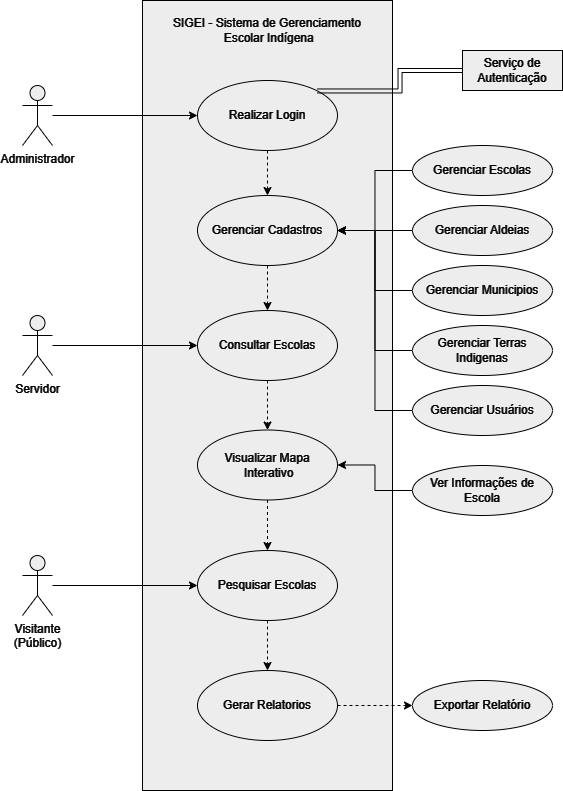
\includegraphics[width=0.85\textwidth]{imagens/diagrama-casos-de-uso.drawio.png}
\caption{Diagrama de casos de uso do SIGEI}
\fonte{Euzébio do Nascimento Oliveira Neto (2026)}
\label{fig:casosdeuso}
\end{figure}

\subsection{Diagrama Entidade-Relacionamento}

O modelo de dados do SIGEI foi projetado para representar as entidades do domínio da educação escolar indígena e seus relacionamentos. As principais entidades identificadas são: \texttt{Escola}, \texttt{Aldeia}, \texttt{TerraIndigena}, \texttt{Municipio} e \texttt{Matricula}. A entidade \texttt{Escola} é central no modelo: está localizada em uma \texttt{Aldeia}, que pertence a uma \texttt{TerraIndigena} e a um \texttt{Municipio}, e registra \texttt{Matricula}s por período letivo.

\begin{figure}[H]
\centering
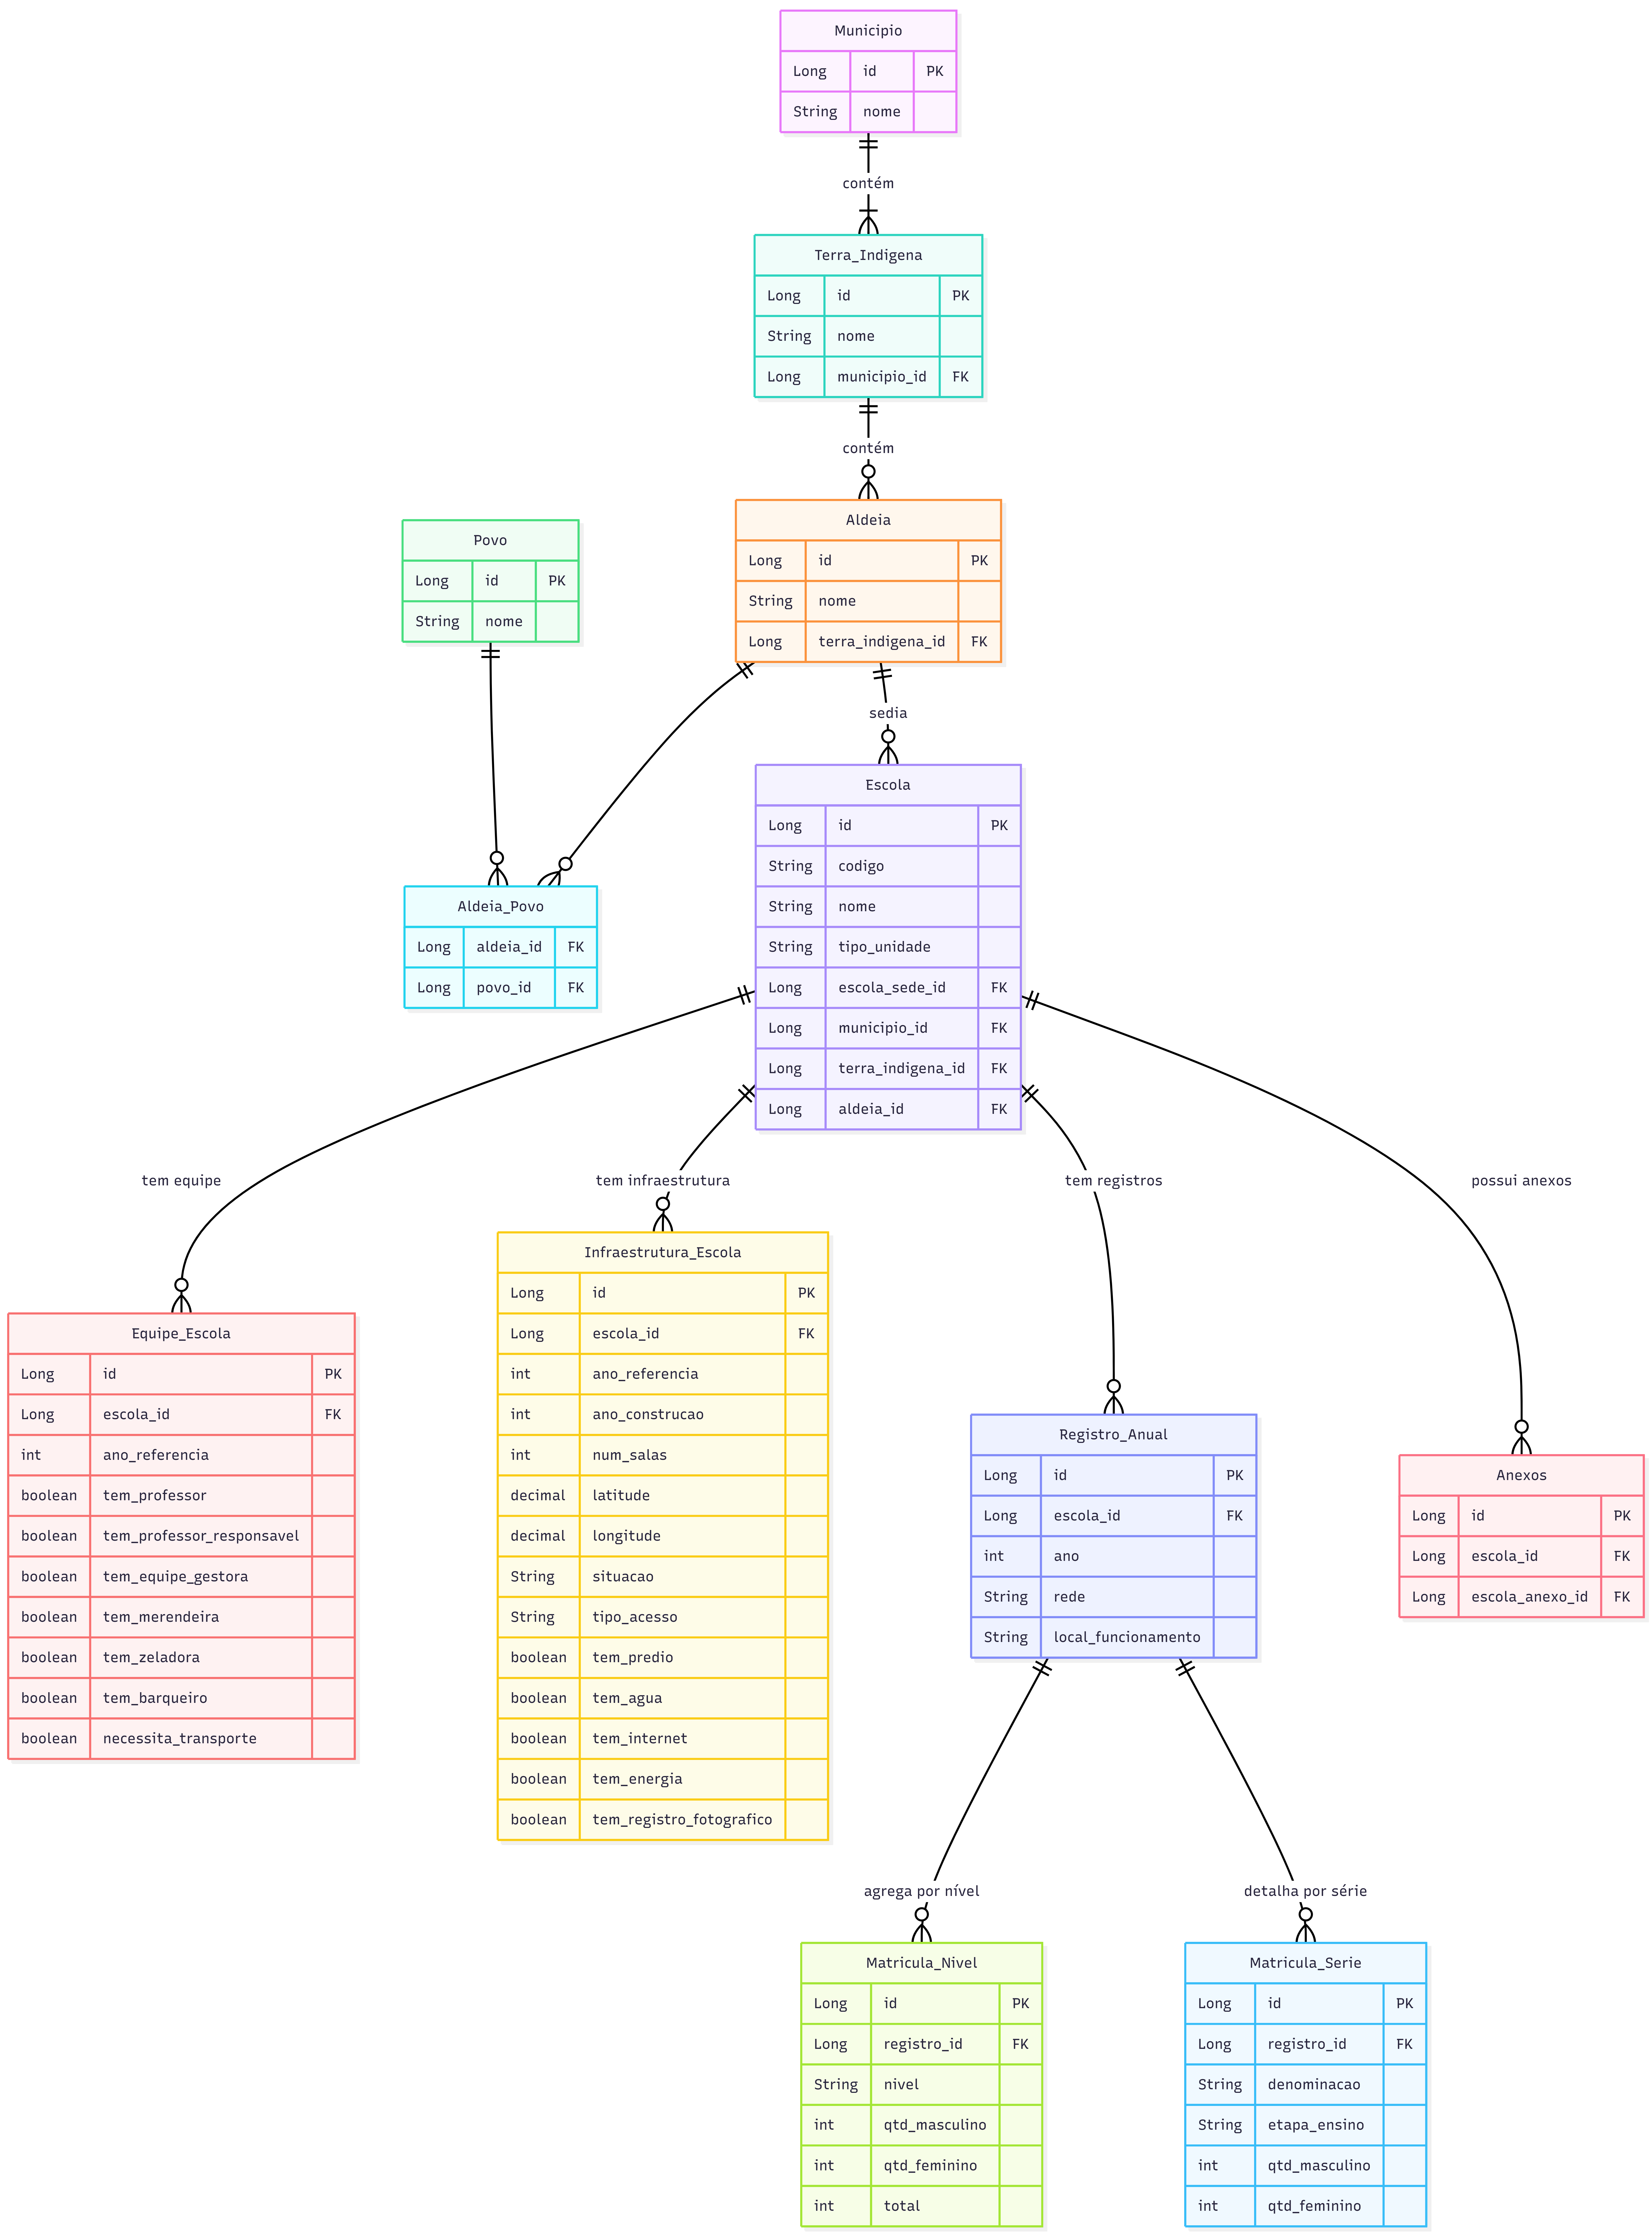
\includegraphics[width=0.90\textwidth]{imagens/SIGEI - ER2-2026-06-26-142013.png}
\caption{Diagrama entidade-relacionamento do SIGEI}
\fonte{Euzébio do Nascimento Oliveira Neto (2026)}
\label{fig:der}
\end{figure}

\subsection{Arquitetura em Camadas}

O SIGEI será projetado seguindo o padrão de arquitetura em camadas, que promove a separação de responsabilidades entre os diferentes componentes do sistema \cite{pressman2016}. As camadas adotadas são:

\begin{alineas}
  \item \textbf{Controller (Controlador):} responsável por receber as requisições HTTP, validar os dados de entrada e delegar o processamento à camada de serviço;
  \item \textbf{Service (Serviço):} concentra a lógica de negócio da aplicação, realizando transformações de dados e coordenando as operações entre diferentes repositórios;
  \item \textbf{Repository (Repositório):} abstrai as operações de acesso ao banco de dados, utilizando a interface \texttt{JpaRepository} do Spring Data JPA;
  \item \textbf{Entity (Entidade):} representa as classes de domínio mapeadas para as tabelas do banco de dados por meio das anotações JPA/Hibernate;
  \item \textbf{DTO (\textit{Data Transfer Object}):} objetos utilizados para a transferência de dados entre as camadas, evitando a exposição direta das entidades na interface da API.
\end{alineas}

\section{Arquitetura do Sistema}

A arquitetura geral do SIGEI seguirá o modelo cliente-servidor, com clara separação entre o \textit{frontend}, o \textit{backend} e o banco de dados. O Quadro~\ref{qua:arq} resume os componentes e as tecnologias adotadas em cada camada.

\begin{table}[H]
\centering
\caption{Arquitetura do SIGEI por camadas}
\label{qua:arq}
\begin{tabularx}{\textwidth}{lX}
\toprule
\textbf{Camada} & \textbf{Tecnologia e responsabilidade} \\
\midrule
\textit{Frontend}       & Angular + TypeScript + Leaflet: interface do usuário, mapa interativo, consumo da API REST \\[4pt]
Comunicação             & API REST via HTTP/JSON: troca de dados entre \textit{frontend} e \textit{backend} \\[4pt]
\textit{Backend}        & Java 17 + Spring Boot + Spring Data JPA + Hibernate: lógica de negócio e persistência \\[4pt]
Banco de Dados          & PostgreSQL: armazenamento relacional dos dados do sistema \\
\bottomrule
\end{tabularx}
\fonte{Euzébio do Nascimento Oliveira Neto (2026)}
\end{table}

\begin{figure}[H]
\centering
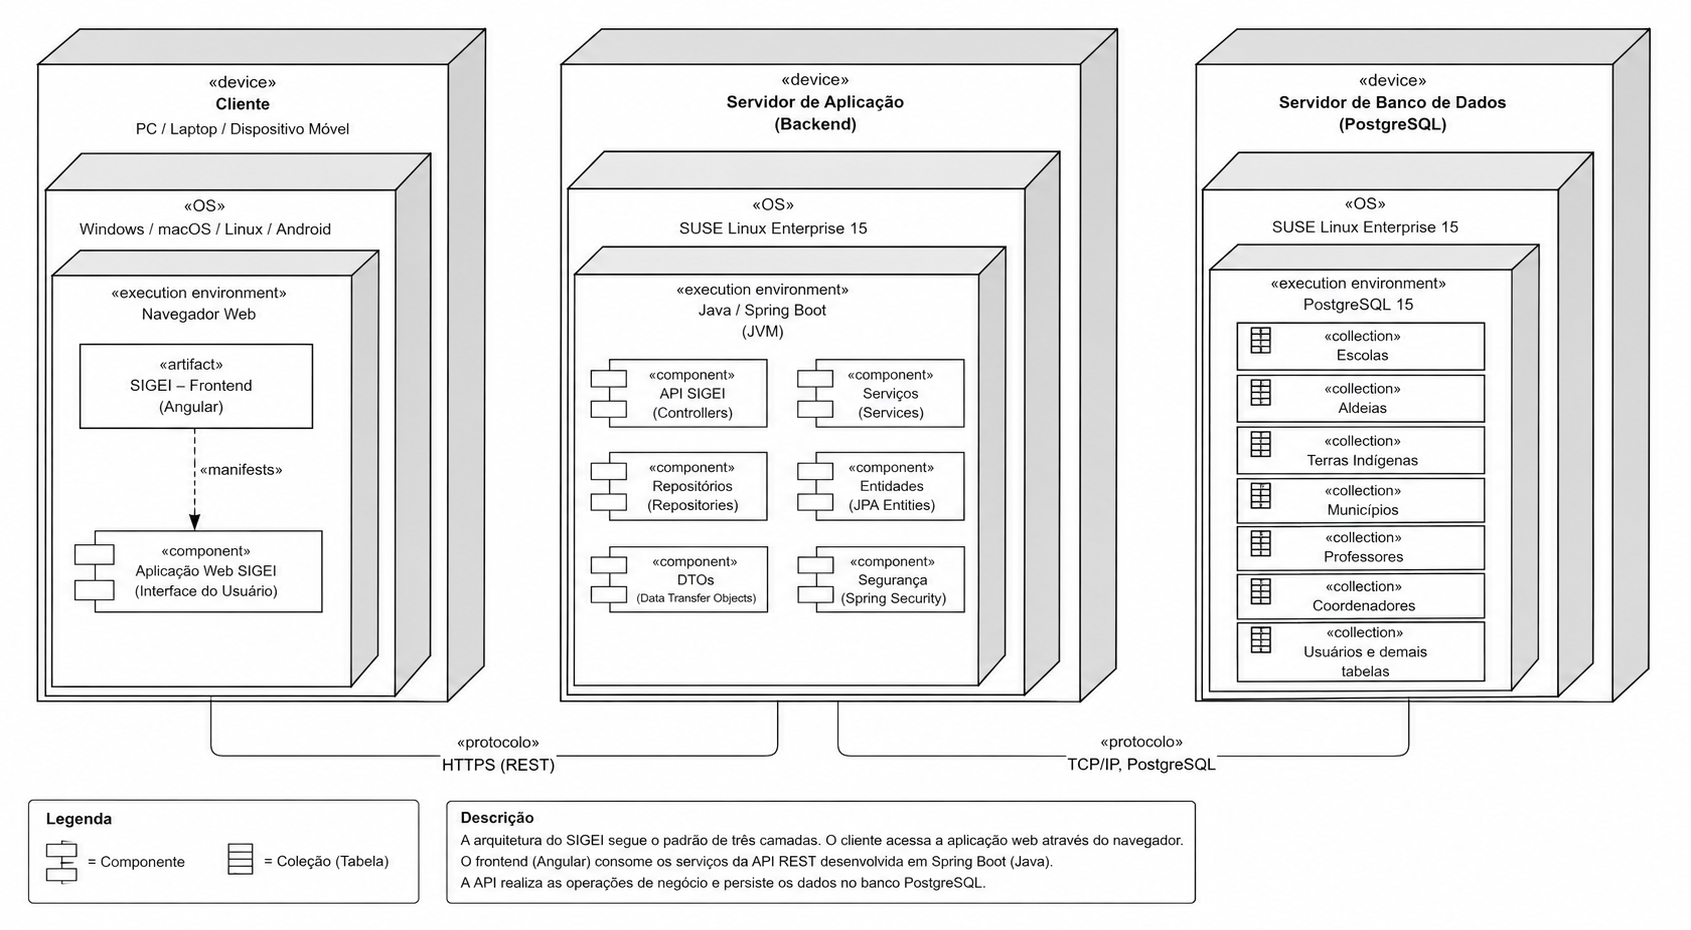
\includegraphics[width=0.75\textwidth]{imagens/diagrama-arquitetura.png}
\caption{Diagrama da arquitetura em camadas do SIGEI}
\fonte{Euzébio do Nascimento Oliveira Neto (2026)}
\label{fig:arquitetura}
\end{figure}

\section{Tecnologias a Serem Utilizadas}

\subsection{\textit{Frontend}: Angular e TypeScript}

No \textit{frontend}, o SIGEI utilizará o framework Angular na versão 16, que proporciona uma estrutura modular e orientada a componentes. A linguagem TypeScript garantirá a tipagem estática do código, contribuindo para a detecção precoce de erros e para a manutenibilidade da aplicação. A biblioteca Leaflet será integrada ao Angular por meio do pacote \texttt{ngx-leaflet}, que fornece uma diretiva Angular para a inicialização e o controle do mapa interativo. Os marcadores geográficos das escolas serão gerados dinamicamente a partir dos dados retornados pela API REST, renderizados sobre uma camada de \textit{tiles} do OpenStreetMap.

\subsection{\textit{Backend}: Java e Spring Boot}

No \textit{backend}, o SIGEI será desenvolvido em Java 17, utilizando o Spring Boot como \textit{framework} principal. A exposição dos \textit{endpoints} da API REST ocorrerá por meio das anotações \texttt{@RestController} e \texttt{@RequestMapping} do Spring MVC. O acesso ao banco de dados será realizado por meio do Spring Data JPA, com o Hibernate como provedor JPA padrão. A validação dos dados de entrada ocorrerá com o \textit{Bean Validation} (JSR-380), por meio das anotações \texttt{@NotNull}, \texttt{@NotBlank} e \texttt{@Size}.

\subsection{Banco de Dados: PostgreSQL}

O banco de dados relacional PostgreSQL será utilizado para o armazenamento de todas as informações gerenciadas pelo SIGEI. O esquema será criado e mantido por meio do Hibernate com a propriedade \texttt{spring.jpa.hibernate.ddl-auto}. As coordenadas geográficas das escolas serão armazenadas como colunas numéricas de precisão dupla (\texttt{DOUBLE PRECISION}) para latitude e longitude.


% CAPÍTULO 4 — DESENVOLVIMENTO E RESULTADOS

\chapter{DESENVOLVIMENTO E RESULTADOS}
\label{cap:desenvolvimento}

Este capítulo descreve o sistema efetivamente implementado a partir do planejamento apresentado no Capítulo~\ref{cap:metodos}. São apresentados a arquitetura adotada no \textit{backend} e no \textit{frontend}, o modelo de dados, os mecanismos de segurança, a interface de programação disponibilizada, as funcionalidades desenvolvidas, a verificação do atendimento aos requisitos e as limitações identificadas.

\section{Visão Geral da Solução}

O SIGEI foi construído como uma aplicação web composta por três elementos independentes: uma API REST desenvolvida em Java com Spring Boot, uma aplicação de página única (SPA) desenvolvida em Angular e um banco de dados relacional PostgreSQL. As fotografias das escolas são armazenadas em um serviço externo de hospedagem de imagens, o Cloudinary, e o banco de dados guarda apenas o endereço de cada imagem.

A aplicação oferece dois modos de acesso. O primeiro é um mapa público, acessível sem autenticação, que apresenta a localização georreferenciada das escolas indígenas do Acre. O segundo é uma área administrativa, restrita a usuários autenticados, na qual são realizados os cadastros, a manutenção do histórico anual das escolas e a consulta aos indicadores consolidados.

Em relação ao planejamento inicial, algumas decisões tecnológicas foram revistas durante a implementação. O \textit{backend} foi desenvolvido em Java 21 com Spring Boot 4, e o \textit{frontend} em Angular 21. O Leaflet passou a ser utilizado diretamente, sem o pacote intermediário \texttt{ngx-leaflet}, o que simplificou a integração com os componentes independentes (\textit{standalone}) do Angular.

\section{Arquitetura Implementada}

\subsection{\textit{Backend}}

O \textit{backend} segue a arquitetura em camadas descrita no Capítulo~\ref{cap:metodos}, na qual cada requisição percorre o fluxo controlador, serviço e repositório \cite{pressman2016}. Os controladores recebem as requisições HTTP e validam os dados de entrada; os serviços concentram as regras de negócio e delimitam as transações; os repositórios, baseados no Spring Data JPA, realizam o acesso ao banco de dados \cite{walls2019}. A conversão entre entidades e objetos de transferência de dados (DTOs) é feita por interfaces do MapStruct, que geram o código de conversão em tempo de compilação. Assim, as entidades JPA nunca são expostas diretamente na API. O Quadro~\ref{qua:pacotes} resume a organização dos pacotes.

\begin{longtable}{p{3.5cm}p{10cm}}
\caption{Organização dos pacotes do \textit{backend}}
\label{qua:pacotes} \\
\toprule
\textbf{Pacote} & \textbf{Responsabilidade} \\
\midrule
\endfirsthead
\toprule
\textbf{Pacote} & \textbf{Responsabilidade} \\
\midrule
\endhead
\midrule
\multicolumn{2}{r}{\small\textit{continua na próxima página}} \\
\endfoot
\bottomrule
\endlastfoot
\texttt{controllers}  & Definição das rotas HTTP, validação da entrada e montagem das respostas. \\[3pt]
\texttt{service}      & Regras de negócio, transações, autenticação, armazenamento de imagens e importação de planilhas. \\[3pt]
\texttt{repository}   & Interfaces Spring Data JPA, consultas personalizadas e agregações dos indicadores. \\[3pt]
\texttt{models}       & Entidades JPA e enumerações do domínio. \\[3pt]
\texttt{dto}          & Contratos de entrada (\textit{request}) e de saída (\textit{response}) da API. \\[3pt]
\texttt{mappers}      & Conversão entre entidades e DTOs com MapStruct. \\[3pt]
\texttt{config}       & Segurança, inicialização de dados e integração com o Cloudinary. \\[3pt]
\texttt{exceptions}   & Exceções da aplicação e tratamento global de erros HTTP. \\[3pt]
\texttt{utils}        & Leitura de planilhas Excel, normalização de coordenadas e contadores de importação. \\
\end{longtable}
\fonte{Euzébio do Nascimento Oliveira Neto (2026)}

O tratamento de erros é centralizado em um componente anotado com \texttt{@RestControllerAdvice}, que converte as exceções em respostas HTTP padronizadas: 400 para dados inválidos, 404 para recursos inexistentes, 409 para violações de integridade referencial e 503 quando o serviço de armazenamento de imagens não está configurado.

\subsection{\textit{Frontend}}

O \textit{frontend} foi construído com componentes independentes (\textit{standalone components}) do Angular, dispensando a declaração de módulos \cite{angular2023}. O código foi organizado em quatro áreas:

\begin{alineas}
  \item \textbf{\texttt{core}:} serviço de autenticação, interceptador HTTP e \textit{guards} de rota;
  \item \textbf{\texttt{domains}:} serviços de acesso à API e modelos de dados, agrupados pelos domínios escolas, territórios e usuários;
  \item \textbf{\texttt{features}:} telas da aplicação, agrupadas em mapa público, autenticação e área administrativa;
  \item \textbf{\texttt{shared}:} componentes visuais reutilizáveis, como cabeçalho e janelas de confirmação.
\end{alineas}

Todas as telas são carregadas sob demanda (\textit{lazy loading}): o navegador baixa o código de cada página apenas quando ela é acessada, o que reduz o tempo de carregamento inicial do mapa público. A aplicação também utiliza a detecção de mudanças sem a biblioteca Zone.js, recurso disponível nas versões recentes do Angular. A estilização foi feita com o \textit{framework} de CSS utilitário Tailwind CSS, que permitiu construir uma interface responsiva a partir de classes aplicadas diretamente nos \textit{templates} \cite{freeman2019}.

\subsection{Implantação}

Tanto o \textit{backend} quanto o \textit{frontend} possuem arquivos \texttt{Dockerfile} e \texttt{docker-compose}, o que permite executar o sistema completo em contêineres. O contêiner do \textit{backend} é acompanhado de um contêiner PostgreSQL com volume persistente. O do \textit{frontend} utiliza o servidor Nginx, configurado para redirecionar as rotas da SPA para o arquivo \texttt{index.html}, aplicar compressão e cabeçalhos de segurança e encaminhar as chamadas à API. As configurações sensíveis, como credenciais do banco de dados, segredo de assinatura dos \textit{tokens} e chaves do Cloudinary, são fornecidas por variáveis de ambiente e não são versionadas no repositório.

% TODO: inserir diagrama de implantação (navegador → Nginx/Angular → API Spring Boot → PostgreSQL e Cloudinary)
% \begin{figure}[H]
% \centering
% \includegraphics[width=0.85\textwidth]{imagens/diagrama-implantacao.png}
% \caption{Diagrama de implantação do SIGEI}
% \fonte{Euzébio do Nascimento Oliveira Neto (2026)}
% \label{fig:implantacao}
% \end{figure}

\section{Modelo de Dados}

O modelo de dados implementado é composto por treze entidades persistidas pelo Hibernate \cite{bauer2015}. As entidades territoriais formam uma hierarquia: \texttt{Municipio} contém \texttt{TerraIndigena}; \texttt{Aldeia} pertence a uma terra indígena e está associada a um \texttt{Povo}; \texttt{Escola} está localizada em uma aldeia. A entidade \texttt{Usuario} armazena as credenciais e o perfil de acesso.

A principal decisão de modelagem foi separar os dados permanentes da escola dos dados que variam a cada ano. A entidade \texttt{Escola} guarda apenas os atributos estáveis: código INEP, nome, tipo de unidade (sede ou anexo) e escola-sede, quando se tratar de anexo. As informações anuais ficam na entidade \texttt{RegistroAnual}, que associa uma escola a um \texttt{AnoReferencia}. Uma restrição de unicidade sobre o par escola e ano impede registros duplicados. Cada registro anual possui:

\begin{alineas}
  \item uma \texttt{EquipeEscola}, que indica a presença de professor responsável, equipe gestora, merendeira, zeladora e barqueiro, além da necessidade de transporte;
  \item uma \texttt{InfraestruturaEscola}, com ano de construção, número de salas, coordenadas geográficas, situação de funcionamento, tipo de acesso, abastecimento de água, energia, internet, existência de prédio e fotografia;
  \item um conjunto de \texttt{MatriculaNivel}, com as matrículas por nível de ensino e por sexo;
  \item um conjunto de \texttt{MatriculaSerie}, com as matrículas por ano ou série, incluindo os ciclos da Educação de Jovens e Adultos.
\end{alineas}

Essa estrutura preserva o histórico de cada unidade escolar: a atualização dos dados de um ano não altera os registros dos anos anteriores. Como as coordenadas ficam na infraestrutura anual, e não na escola, eventuais mudanças de local de funcionamento também são preservadas no histórico. Os relacionamentos entre o registro anual e seus dependentes utilizam exclusão em cascata, de modo que a remoção de um registro elimina também a equipe, a infraestrutura e as matrículas correspondentes.

% TODO: substituir pelo diagrama ER atualizado (13 entidades). O arquivo sigei-backend/docs/MODELO_ER.md
% contém o diagrama em Mermaid gerado a partir das entidades JPA.
% \begin{figure}[H]
% \centering
% \includegraphics[width=0.95\textwidth]{imagens/modelo-er-implementado.png}
% \caption{Modelo entidade-relacionamento implementado}
% \fonte{Euzébio do Nascimento Oliveira Neto (2026)}
% \label{fig:erimplementado}
% \end{figure}

O esquema do banco é gerado e atualizado pelo Hibernate a partir das entidades, conforme a propriedade \texttt{spring.jpa.hibernate.ddl-auto}. As coordenadas geográficas são armazenadas como números de precisão dupla, conforme previsto no planejamento.

\section{Segurança e Controle de Acesso}

A autenticação foi implementada com o Spring Security em modo sem estado (\textit{stateless}), com \textit{tokens} JWT (\textit{JSON Web Token}). O fluxo ocorre da seguinte forma:

\begin{alineas}
  \item o usuário informa e-mail e senha na tela de \textit{login};
  \item o \textit{backend} verifica se o usuário está ativo e compara a senha com o valor armazenado, cifrado com o algoritmo BCrypt;
  \item em caso de sucesso, é emitido um \textit{token} assinado com validade padrão de 24 horas, contendo a identificação e o perfil do usuário;
  \item o \textit{frontend} armazena o \textit{token} e o envia no cabeçalho \texttt{Authorization} de cada requisição por meio de um interceptador HTTP;
  \item a cada requisição, um filtro do \textit{backend} valida o \textit{token} e consulta novamente o cadastro do usuário, de modo que a desativação de uma conta tem efeito imediato.
\end{alineas}

Foram definidos dois perfis de acesso, correspondentes aos atores do diagrama de casos de uso (Figura~\ref{fig:casosdeuso}): \texttt{ADMIN}, equivalente ao Gestor, e \texttt{USUARIO}, equivalente ao Consulente. O Quadro~\ref{qua:permissoes} apresenta as regras de autorização aplicadas.

\begin{longtable}{p{6cm}p{7.5cm}}
\caption{Regras de autorização da API}
\label{qua:permissoes} \\
\toprule
\textbf{Requisição} & \textbf{Acesso} \\
\midrule
\endfirsthead
\toprule
\textbf{Requisição} & \textbf{Acesso} \\
\midrule
\endhead
\midrule
\multicolumn{2}{r}{\small\textit{continua na próxima página}} \\
\endfoot
\bottomrule
\endlastfoot
\textit{Login}, verificação de saúde e documentação da API & Público \\[3pt]
Consulta às infraestruturas (dados do mapa)              & Público \\[3pt]
Alteração da própria senha                                 & Qualquer usuário autenticado \\[3pt]
Demais consultas (\texttt{GET})                            & Perfis \texttt{ADMIN} e \texttt{USUARIO} \\[3pt]
Inclusões, alterações e exclusões                          & Somente \texttt{ADMIN} \\
\end{longtable}
\fonte{Euzébio do Nascimento Oliveira Neto (2026)}

O administrador inicial é criado automaticamente na primeira execução do sistema com a troca de senha marcada como obrigatória. Enquanto a senha não é alterada, o \textit{token} emitido concede apenas a permissão de trocá-la, e o \textit{frontend} redireciona o usuário para a tela correspondente. O mesmo ocorre com os usuários cadastrados por um administrador.

No \textit{frontend}, \textit{guards} de rota impedem a navegação para páginas não permitidas ao perfil do usuário e ocultam os botões de edição para o perfil \texttt{USUARIO}. Essa verificação serve à usabilidade. A garantia efetiva de acesso é feita no \textit{backend}, que rejeita com os códigos 401 ou 403 qualquer requisição não autorizada, independentemente da interface utilizada. O compartilhamento de recursos entre origens (CORS) é restrito às origens configuradas para o \textit{frontend}.

\section{Interface de Programação da Aplicação}

A API segue o estilo arquitetural REST \cite{fielding2000}, com recursos identificados por URIs, operações expressas pelos verbos HTTP e representação em JSON \cite{richardson2013}. O Quadro~\ref{qua:endpoints} resume os recursos disponibilizados.

\begin{longtable}{p{4cm}p{9.5cm}}
\caption{Recursos da API REST do SIGEI}
\label{qua:endpoints} \\
\toprule
\textbf{Recurso} & \textbf{Operações} \\
\midrule
\endfirsthead
\toprule
\textbf{Recurso} & \textbf{Operações} \\
\midrule
\endhead
\midrule
\multicolumn{2}{r}{\small\textit{continua na próxima página}} \\
\endfoot
\bottomrule
\endlastfoot
\texttt{/municipio}          & Cadastro e consulta; estatísticas por município. \\[3pt]
\texttt{/terra}              & Cadastro e consulta de terras indígenas; estatísticas. \\[3pt]
\texttt{/aldeia}, \texttt{/povo} & Cadastro e consulta. \\[3pt]
\texttt{/escola}             & Cadastro e consulta; detalhe da escola com o registro anual mais recente. \\[3pt]
\texttt{/anos}               & Cadastro dos anos de referência. \\[3pt]
\texttt{/registroAnual}      & Cadastro; consulta por ano, por escola e ano, e histórico de uma escola em um intervalo de anos. \\[3pt]
\texttt{/equipe}             & Inclusão e alteração da equipe de um registro anual. \\[3pt]
\texttt{/infraestrutura}     & Cadastro e consulta; consulta por ano; envio de fotografia. \\[3pt]
\texttt{/matriculaNivel}, \texttt{/matriculaSerie} & Cadastro das matrículas de um registro anual. \\[3pt]
\texttt{/atualizacao-anual}  & Abertura de um novo ano de referência. \\[3pt]
\texttt{/importacoes}        & Importação de planilhas de infraestrutura e de matrículas. \\[3pt]
\texttt{/dashboard}          & Indicadores consolidados, com ano opcional. \\[3pt]
\texttt{/usuario}            & Cadastro e consulta de usuários. \\[3pt]
\texttt{/auth}               & \textit{Login} e alteração de senha. \\
\end{longtable}
\fonte{Euzébio do Nascimento Oliveira Neto (2026)}

A API é documentada automaticamente com a especificação OpenAPI, gerada pela biblioteca Springdoc a partir de anotações nos controladores. A documentação interativa fica disponível na interface Swagger UI, que permite consultar os contratos de entrada e saída e testar as operações diretamente pelo navegador.

\section{Funcionalidades Desenvolvidas}

\subsection{Mapa Público Interativo}

O mapa público é a página inicial do sistema e não exige autenticação. Ele foi desenvolvido com a biblioteca Leaflet \cite{leaflet2023} e apresenta um marcador para cada escola com coordenadas cadastradas, posicionado sobre o território do Acre. A cor do marcador indica a situação da unidade: verde para escolas em funcionamento e vermelho para escolas paralisadas. Essa codificação permite identificar visualmente a distribuição espacial das unidades que demandam atenção \cite{longley2013}.

O usuário pode alternar entre quatro camadas de fundo (mapa padrão do OpenStreetMap, imagem de satélite, relevo e tema escuro), pesquisar escolas por nome ou código INEP e aplicar filtros por situação, tipo de acesso (terrestre, fluvial, aéreo ou misto), disponibilidade de internet e existência de prédio. Ao selecionar uma escola, o mapa é centralizado sobre ela e exibe uma janela com fotografia, código INEP, situação, tipo de acesso e indicadores de infraestrutura.

% TODO: inserir captura de tela do mapa público
% \begin{figure}[H]
% \centering
% 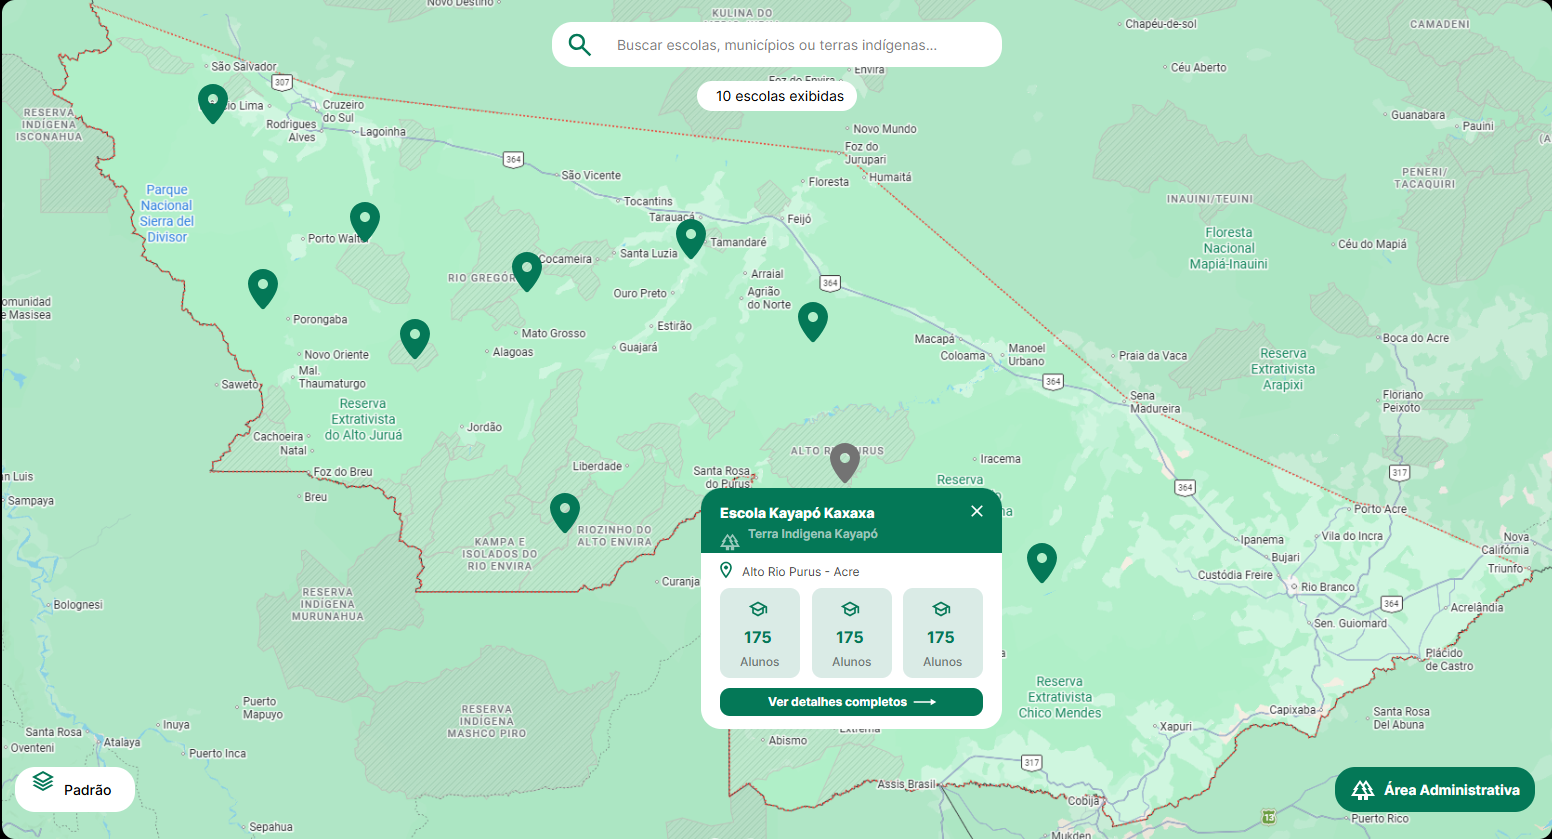
\includegraphics[width=0.95\textwidth]{imagens/tela-mapa.png}
% \caption{Mapa público do SIGEI}
% \fonte{Euzébio do Nascimento Oliveira Neto (2026)}
% \label{fig:telamapa}
% \end{figure}

\subsection{Painel de Indicadores}

Após a autenticação, o usuário é direcionado a um painel (\textit{dashboard}) que consolida as informações de um ano de referência, por padrão o mais recente. O painel apresenta:

\begin{alineas}
  \item totais de escolas, matrículas, municípios e terras indígenas;
  \item evolução do número de matrículas e de escolas ao longo dos anos cadastrados;
  \item distribuição das matrículas por nível de ensino;
  \item percentual de escolas com internet, energia elétrica e prédio próprio;
  \item quantidade de escolas por município e por situação de funcionamento.
\end{alineas}

Os indicadores são calculados no banco de dados por consultas de agregação, e o \textit{frontend} apenas recebe os valores consolidados. O painel atende ao objetivo de disponibilizar informações gerenciais aos gestores da SEE/AC.

% TODO: inserir captura de tela do dashboard
% \begin{figure}[H]
% \centering
% \includegraphics[width=0.95\textwidth]{imagens/tela-dashboard.png}
% \caption{Painel de indicadores}
% \fonte{Euzébio do Nascimento Oliveira Neto (2026)}
% \label{fig:teladashboard}
% \end{figure}

\subsection{Cadastros Territoriais}

A área administrativa oferece telas de listagem, pesquisa e manutenção para terras indígenas, aldeias e povos. Todas as exclusões exigem confirmação prévia. Os municípios do Acre são cadastrados automaticamente pelo sistema na inicialização, e a tela correspondente apresenta, para cada município, a quantidade de terras indígenas, aldeias e escolas associadas.

\subsection{Cadastro de Escolas}

Por envolver muitas informações, o cadastro de escolas foi dividido em sete etapas sequenciais, cada uma validada antes do avanço para a seguinte:

\begin{alineas}
  \item dados da escola: código INEP, nome, tipo de unidade, aldeia e, para anexos, a escola-sede;
  \item registro anual: ano de referência, rede de ensino e local de funcionamento;
  \item equipe escolar;
  \item infraestrutura, com coordenadas geográficas e envio opcional de fotografia;
  \item matrículas por nível de ensino (Educação Infantil, Ensino Fundamental -- anos iniciais e finais, Ensino Médio, EJA e AEE), separadas por sexo;
  \item matrículas por ano ou série, do 1.º ano do Ensino Fundamental à 3.ª série do Ensino Médio, além dos ciclos da EJA;
  \item revisão dos dados antes da gravação.
\end{alineas}

Os totais de matrículas são calculados automaticamente pela interface à medida que as quantidades são informadas. A mesma tela é utilizada para a edição, quando carrega os dados já cadastrados da escola.

% TODO: inserir captura de tela de uma etapa do cadastro de escolas
% \begin{figure}[H]
% \centering
% \includegraphics[width=0.95\textwidth]{imagens/tela-cadastro-escola.png}
% \caption{Cadastro de escolas em etapas}
% \fonte{Euzébio do Nascimento Oliveira Neto (2026)}
% \label{fig:telacadastroescola}
% \end{figure}

\subsection{Histórico Anual e Abertura de Novo Ano}

A tela de histórico permite consultar os registros de duas formas: todos os registros de um ano ou a evolução de uma escola específica em um intervalo de anos. A partir dela, o administrador pode editar os dados de um ano específico ou cadastrar retroativamente um ano anterior, sem afetar os demais registros da escola.

Para a virada do ano letivo, foi implementada a operação de abertura de novo ano. Ela cria o ano de referência seguinte ao mais recente e, para cada escola, gera um novo registro anual copiando rede, local de funcionamento, equipe, infraestrutura e matrículas do último registro existente. A operação é executada em uma única transação no banco de dados. O gestor passa então a atualizar apenas as informações que mudaram, sem recadastrar as escolas.

\subsection{Carga Inicial e Importação de Planilhas}

Para aproveitar os dados já existentes na SEE/AC, que antes estavam dispersos em planilhas eletrônicas, foi desenvolvido um módulo de importação com a biblioteca Apache POI. Ele lê a planilha de infraestrutura e a planilha de matrículas do censo escolar, normaliza os nomes, converte as coordenadas geográficas e identifica as escolas. As terras indígenas, povos, aldeias e escolas ainda não cadastrados são criados, e os registros anuais correspondentes são criados ou atualizados. Ao final, informa a quantidade de linhas processadas e os erros encontrados.

Na primeira execução do sistema com o banco de dados vazio, essa importação é realizada automaticamente. Assim, o sistema já é disponibilizado com os dados das escolas indígenas carregados. A importação também está disponível pela API para uso posterior.

\subsection{Gestão de Usuários e Preferências}

Os administradores podem cadastrar, editar, ativar e desativar usuários e definir o perfil de acesso de cada um. Cada usuário pode ainda ajustar preferências de exibição do mapa, como a camada de fundo padrão, a abertura das janelas ao passar o cursor e a exibição de fotografias. Essas preferências são armazenadas no próprio navegador.

\section{Atendimento aos Requisitos}

O Quadro~\ref{qua:atendimentorf} relaciona os requisitos funcionais apresentados no Quadro~\ref{qua:rf} às funcionalidades implementadas.

\begin{longtable}{p{1.5cm}p{3cm}p{2.2cm}p{6.8cm}}
\caption{Atendimento aos requisitos funcionais}
\label{qua:atendimentorf} \\
\toprule
\textbf{Código} & \textbf{Requisito} & \textbf{Situação} & \textbf{Implementação} \\
\midrule
\endfirsthead
\toprule
\textbf{Código} & \textbf{Requisito} & \textbf{Situação} & \textbf{Implementação} \\
\midrule
\endhead
\midrule
\multicolumn{4}{r}{\small\textit{continua na próxima página}} \\
\endfoot
\bottomrule
\endlastfoot
RF01 & Cadastrar escola          & Atendido & Cadastro em sete etapas, com dados anuais, infraestrutura, fotografia e matrículas. \\[3pt]
RF02 & Editar escola             & Atendido & Edição dos dados permanentes e de qualquer ano do histórico. \\[3pt]
RF03 & Excluir escola            & Atendido & Exclusão com confirmação prévia. \\[3pt]
RF04 & Visualizar no mapa        & Atendido & Mapa Leaflet com marcadores diferenciados por situação. \\[3pt]
RF05 & Gerenciar aldeias         & Atendido & Cadastro, edição, consulta e exclusão, vinculados à terra indígena e ao povo. \\[3pt]
RF06 & Gerenciar municípios      & Atendido & Carga automática dos municípios do Acre e consulta com estatísticas; API com operações completas. \\[3pt]
RF07 & Gerenciar terras indígenas & Atendido & Cadastro, edição, consulta e exclusão. \\[3pt]
RF08 & Gerar relatórios          & Parcial  & Indicadores consolidados no painel; exportação de relatórios em arquivo não implementada. \\[3pt]
RF09 & Registrar matrículas      & Atendido & Matrículas por nível e por série, por sexo, em cada ano de referência. \\[3pt]
RF10 & Consultar mapa interativo & Atendido & Busca, filtros e janela de informações por escola. \\
\end{longtable}
\fonte{Euzébio do Nascimento Oliveira Neto (2026)}

Quanto aos requisitos não funcionais, a interface foi construída com classes responsivas do Tailwind CSS e se adapta a telas de dispositivos móveis (RNF01). O sistema é acessado por navegador, sem instalação de \textit{software} adicional (RNF02). O controle de acesso é garantido pela autenticação JWT e pelos perfis descritos na seção anterior (RNF03). A integridade dos dados é assegurada por chaves estrangeiras, restrições de unicidade e validações com \textit{Bean Validation} na camada de aplicação (RNF06). O desempenho do mapa (RNF04) e a usabilidade (RNF05) não foram submetidos a medições ou testes formais com usuários, o que fica registrado como trabalho futuro.

\section{Testes}

A verificação do \textit{backend} foi realizada com testes automatizados escritos com JUnit 5 e Mockito, organizados em 27 classes de teste que espelham os pacotes da aplicação \cite{sommerville2019}. Os testes de serviço isolam as regras de negócio por meio de objetos simulados (\textit{mocks}) dos repositórios. Os testes de repositório utilizam a anotação \texttt{@DataJpaTest} com um banco de dados H2 em memória, verificando os mapeamentos, as consultas personalizadas e as agregações do painel de indicadores. Também foram testados o inicializador de municípios e o histórico anual das escolas.

Além dos testes automatizados, as rotas da API foram verificadas manualmente com uma coleção de requisições da ferramenta Bruno, e as telas do \textit{frontend} foram validadas por testes funcionais manuais durante cada incremento de desenvolvimento. O \textit{frontend} possui o executor de testes Vitest configurado, mas ainda não conta com testes automatizados.

\section{Limitações e Trabalhos Futuros}

Durante o desenvolvimento, foram identificadas as seguintes limitações, que orientam a continuidade do projeto:

\begin{alineas}
  \item a exportação de relatórios em formatos como PDF ou planilha ainda não foi implementada;
  \item o módulo de importação foi construído para o leiaute das planilhas disponibilizadas pela SEE/AC, com colunas e ano de referência fixos, e precisa ser generalizado para cargas de anos futuros;
  \item o cadastro de uma escola é gravado por uma sequência de requisições à API, e não por uma única transação, de modo que uma falha intermediária pode deixar o cadastro incompleto até nova gravação;
  \item não há renovação automática do \textit{token} de acesso; após o período de validade, o usuário precisa se autenticar novamente;
  \item o \textit{frontend} não possui testes automatizados, e não foram realizadas avaliações formais de desempenho e de usabilidade com os gestores da SEE/AC;
  \item o esquema do banco de dados é mantido pelo Hibernate, e a adoção de uma ferramenta de versionamento de esquema, como Flyway, é recomendável antes do uso em produção.
\end{alineas}



% CAPÍTULO 5 — CRONOGRAMA

\chapter{CRONOGRAMA}
\label{cap:cronograma}

O cronograma de execução do projeto foi elaborado considerando as etapas previstas na metodologia de desenvolvimento incremental adotada, distribuídas ao longo do segundo semestre de 2026, conforme demonstrado na Tabela 4.

\begin{longtable}{p{6.5cm}*{6}{c}}
\caption{Cronograma de atividades do TCC}
\label{qua:cronograma} \\
\toprule
\textbf{Atividade} & \textbf{Maio} & \textbf{Jun} & \textbf{Jul} & \textbf{Ago} & \textbf{Set} & \textbf{Out} \\
\midrule
\endfirsthead
\toprule
\textbf{Atividade} & \textbf{Maio} & \textbf{Jun} & \textbf{Jul} & \textbf{Ago} & \textbf{Set} & \textbf{Out} \\
\midrule
\endhead
\midrule
\multicolumn{7}{r}{\small\textit{continua na próxima página}} \\
\endfoot
\bottomrule
\endlastfoot
Revisão bibliográfica                    & $\bullet$ & $\bullet$ &            &            &            &            \\[3pt]
Levantamento e validação de requisitos   & $\bullet$ & $\bullet$ &            &            &            &            \\[3pt]
Modelagem do banco de dados              &           & $\bullet$ & $\bullet$  &            &            &            \\[3pt]
Implementação do \textit{backend}        &           & $\bullet$ & $\bullet$  & $\bullet$  &            &            \\[3pt]
Implementação do \textit{frontend}       &           &           & $\bullet$  & $\bullet$  &            &            \\[3pt]
Integração \textit{frontend}/\textit{backend} &      &           &            & $\bullet$  & $\bullet$  &            \\[3pt]
Testes e correções                       &           &           &            & $\bullet$  & $\bullet$  &            \\[3pt]
Redação do TCC                           & $\bullet$ & $\bullet$ & $\bullet$  & $\bullet$  & $\bullet$  &            \\[3pt]
Revisão final e entrega do TCC           &           &           &            &            & $\bullet$  & $\bullet$  \\[3pt]
Apresentação à banca                     &           &           &            &            &            & $\bullet$  \\
\end{longtable}
\fonte{Euzébio do Nascimento Oliveira Neto (2026)}


% REFERÊNCIAS

\postextual
\bibliography{refs}

\end{document}